% ============================================================
% sections/ch07-casscf.tex —— 第 7 章 CASSCF：当一个行列式不够时怎么办？
% 页数配额：6 页（±1）。数值只取自 data/h2m_pes.csv 与 data/h2m_occupations.csv。
% ============================================================

\section{CASSCF：当一个行列式不够时怎么办？}
\label{ch:07:sec:title}

% ---- 1. 问题链 ----
\begin{problemchain}
\textbf{上一章留下的问题：}CC 在强静态相关下失效。\\
\textbf{本章为什么存在：}用活性空间同时优化轨道与 CI 系数，把静态相关显式容纳进波函数。\\
\textbf{本章留下的新问题：}CASSCF 缺动态相关。
\end{problemchain}

% ---- 2. 方法卡片 ----
\begin{methodcard}
\textbf{方法}：完全活性空间自洽场（complete active space SCF，CASSCF）\quad
\textbf{文献}：\citep{roos1980,helgaker2000,szabo1996}\\
\textbf{核心近似}：选定活性空间内做全 CI，并把轨道与 CI 系数联合优化\\
\textbf{关键方程}：式~\eqref{ch:07:eq:casscf-wavefunction}（CASSCF 波函数）\\
\textbf{ORCA 关键词}：\texttt{! CASSCF def2-TZVPP TightSCF}，
并在 \texttt{\%casscf} 中写 \texttt{nel 8 norb 8 mult 1 nroots 1}\\
\textbf{成本标度}：$\mathcal{O}(N^4)$ 的积分变换，加上活性空间行列式数的指数增长\\
\textbf{能否变分 / 尺寸一致}：是 / 是\\
\textbf{典型失效}：活性空间选择不当、缺动态相关、多根近简并时的根翻转
\end{methodcard}

% ---- 3. 正文 ----
\subsection{静态相关与近简并}
\label{ch:07:sec:static}

第 6 章的 CCSD(T) 以单个 HF 行列式为参考。只要这个行列式在真实波函数中占绝对主导，指数拟设就能有效地收拾剩余的动态相关；但当两个或多个行列式近简并时，参考态本身就不再是好的零阶描述。此时电子不是“成对瞬时回避”，而是同时在几个近简并的组态之间分布，这类相关称为\textbf{静态相关}（static correlation），也称非动态相关。

最小的模型是两个近简并组态的混合：
\begin{equation}
\ket{\Psi}=c_1\ket{\Phi_1}+c_2\ket{\Phi_2},
\qquad
|c_1|^2+|c_2|^2=1 .
\label{ch:07:eq:static-two-det}
\end{equation}
若 $\Phi_1$ 与 $\Phi_2$ 能量相同，变分解给出 $c_1=\pm c_2=1/\sqrt{2}$，两个组态权重各半。式~\eqref{ch:07:eq:static-two-det} 的行列式系数是\textbf{分数}的，任何单行列式方法都无法描述；MP2 与 CCSD(T) 的分母在近简并时趋于零，微扰修正随之发散。H$_2^-$ 的拉伸区就是这种情形：三个电子分布在成键 $\sigma$ 与反键 $\sigma^*$ 两个近简并轨道上，单参考图像失效。第 5 章的 CI 能容纳式~\eqref{ch:07:eq:static-two-det}，但截断 CI 不尺寸一致；CASSCF 则把“选哪些行列式”这件事交给一个受控的活性空间。

\subsection{活性空间的概念}
\label{ch:07:sec:active-space}

CASSCF 把轨道分成三组：\textbf{非活性}（inactive）轨道始终双占据，\textbf{活性}（active）轨道上的电子做全 CI，\textbf{虚}（virtual）轨道始终空着。活性空间用两个数标记：
\begin{equation}
\mathrm{CAS}(n_{\mathrm{el}},n_{\mathrm{orb}}):
\qquad
n_{\mathrm{el}}=\sum_{p\in\mathcal{A}} n_p,
\qquad
|\mathcal{A}|=n_{\mathrm{orb}},
\label{ch:07:eq:active-space}
\end{equation}
其中 $\mathcal{A}$ 是活性轨道集合，$n_p$ 是轨道 $p$ 的自然占据数。式~\eqref{ch:07:eq:active-space} 只规定“多少电子、多少轨道”，不预先规定哪些组态；活性空间内的所有组态一视同仁，这正是“完全”（complete）的含义。

对 H$_2^-$，最小且物理的活性空间是 CAS(3,2)：三个电子占据成键 $\sigma$ 与反键 $\sigma^*$ 两个轨道。两个空间轨道、三个电子共给出四个行列式，足以描述 $\sigma$ 与 $\sigma^*$ 之间的近简并。对 CH$_4$，常用 CAS(8,8)：八个价电子进入四条成键轨道与四条反键轨道，用来检验弱静态相关。活性空间越小，计算越便宜，但越可能漏掉重要的近简并组态；这个取舍是 CASSCF 最核心的实际问题。

\subsection{CASSCF 波函数}
\label{ch:07:sec:wavefunction}

在活性空间内，CASSCF 波函数写成所有活性组态行列式的线性组合：
\begin{equation}
\ket{\Psi_{\mathrm{CAS}}}
=\sum_{I\in\mathcal{A}} c_I\ket{\Phi_I},
\qquad
\ket{\Phi_I}
=\Big(\prod_{i\in\mathrm{inact}}\op{a}_i^\dagger\op{a}_{\bar i}^\dagger\Big)
\ket{0}_{\mathrm{act}},
\label{ch:07:eq:casscf-wavefunction}
\end{equation}
其中 $\ket{\Phi_I}$ 由非活性轨道的双占据与活性空间的一个组态构成，$c_I$ 是 CI 系数。与第 5 章的 CI 不同，式~\eqref{ch:07:eq:casscf-wavefunction} 的轨道本身也是变分参数：它们不再固定为 HF 轨道，而是随 $c_I$ 一起调整。

能量是式~\eqref{ch:07:eq:casscf-wavefunction} 的期望值：
\begin{equation}
E_{\mathrm{CAS}}
=\frac{\bracket{\Psi_{\mathrm{CAS}}|\op{H}|\Psi_{\mathrm{CAS}}}}
{\braket{\Psi_{\mathrm{CAS}}|\Psi_{\mathrm{CAS}}}} .
\label{ch:07:eq:casscf-energy}
\end{equation}
式~\eqref{ch:07:eq:casscf-energy} 对轨道与 CI 系数同时变分，因此 CASSCF 是变分的，且对给定活性空间给出该空间内的最优能量。注意“最优”只相对于所选活性空间；丢掉的空间不会因为轨道优化而回来。

\subsection{轨道旋转与 CI 的联合优化}
\label{ch:07:sec:orbital-ci}

轨道优化用一族幺正变换参数化。定义反厄米的轨道旋转生成元
\begin{equation}
\op{\kappa}=\sum_{p,q}\kappa_{pq}\,\op{a}_p^\dagger\op{a}_q,
\qquad
\kappa_{pq}=-\kappa_{qp}^{*},
\label{ch:07:eq:orbital-generator}
\end{equation}
其中 $p,q$ 取遍所有轨道。指数化后得到幺正变换
\begin{equation}
\op{U}(\boldsymbol{\kappa})=\ee^{\op{\kappa}},
\qquad
\ket{\tilde p}=\op{U}\ket{p}.
\label{ch:07:eq:orbital-rotation}
\end{equation}
式~\eqref{ch:07:eq:orbital-rotation} 保持轨道正交归一，因此不会破坏波函数的反对称性；$\kappa_{pq}$ 中只有非冗余分量（非活性--活性、活性--虚、非活性--虚）需要优化，活性--活性之间的旋转不改变 CASSCF 波函数。

固定轨道时，CI 系数由活性空间的本征值问题给出：
\begin{equation}
\sum_{J\in\mathcal{A}}
\bracket{\Phi_I|\op{H}_{\mathrm{act}}|\Phi_J}\,c_J
=E\,c_I ,
\qquad I\in\mathcal{A},
\label{ch:07:eq:ci-eigen}
\end{equation}
其中 $\op{H}_{\mathrm{act}}$ 是投影到活性组态空间的有效 Hamiltonian。式~\eqref{ch:07:eq:ci-eigen} 就是“在活性空间内做全 CI”；它的维数随活性轨道数指数增长，这是 CASSCF 成本的第一部分。

轨道与 CI 的耦合条件是能量对轨道旋转的梯度为零：
\begin{equation}
\frac{\partial E_{\mathrm{CAS}}}{\partial \kappa_{pq}}=0
\quad\Longleftrightarrow\quad
\bracket{\Psi_{\mathrm{CAS}}|[\op{H},\op{a}_p^\dagger\op{a}_q]|\Psi_{\mathrm{CAS}}}=0 .
\label{ch:07:eq:orbital-ci-gradient}
\end{equation}
式~\eqref{ch:07:eq:orbital-generator}--\eqref{ch:07:eq:orbital-ci-gradient} 说明 CASSCF 不是“先做 CI 再优化轨道”的一次性流程，而是两个相互依赖的变分问题：给定轨道解式~\eqref{ch:07:eq:ci-eigen} 得到 $c_I$，再用式~\eqref{ch:07:eq:orbital-ci-gradient} 更新轨道，如此交替直至梯度收敛。实际程序常把两步合成 Super-CI 或二阶方法加速，但数学结构不变。

联合优化也带来新的困难。式~\eqref{ch:07:eq:casscf-energy} 是高度非线性的，可能存在多个局部极小；不同的初始轨道可能收敛到不同的解。活性空间内的近简并还会让不同根的能量顺序在扫描中交换，即\textbf{根翻转}（root flip）。因此 CASSCF 势能曲线必须检查相邻点的能量连续性，并尽量用上一点的轨道作初猜。

\subsection{态平均}
\label{ch:07:sec:state-average}

当需要同时描述多个电子态（例如激发态、或避免某一根在扫描中翻转）时，可以对若干根做\textbf{态平均}（state averaging）。设第 $k$ 根的能量为 $E_k$，权重为 $w_k$，则优化的目标是
\begin{equation}
E_{\mathrm{avg}}=\sum_{k=1}^{n_{\mathrm{root}}} w_k E_k,
\qquad
\sum_{k=1}^{n_{\mathrm{root}}} w_k=1 .
\label{ch:07:eq:state-average}
\end{equation}
式~\eqref{ch:07:eq:state-average} 让同一套轨道同时服务于多个态，通常取等权重。态平均能给出平滑的势能曲线，避免某一根因轨道跟随而跳变；代价是每个态的能量都不是该态单独优化时的最低值。

这一点在 H$_2^-$ 的数据解读中极其重要。本书全部 H$_2^-$ CASSCF 计算都取 \texttt{nroots 1}，即只优化基态一根；若改用 \texttt{nroots 2} 做态平均，得到的“基态”其实是两个态的平均，占据数会被人为地摊成 1.5/1.5。那种 1.5/1.5 不是基态的静态相关证据，本书不使用，也不把它写进任何表格。

\subsection{活性空间怎么选}
\label{ch:07:sec:active-choice}

活性空间的选择没有唯一答案，但有可操作的检查顺序。第一，按化学直觉选：断键涉及成键/反键对，过渡金属涉及 $d$ 壳层与配体轨道，孤对电子与空轨道也常需加入。第二，看自然占据数：式~\eqref{ch:07:eq:casscf-wavefunction} 收敛后，明显偏离 0 或 2 的活性轨道通常必须保留；把占据数接近 0 或 2 的轨道移出活性空间往往影响很小。第三，做稳定性检查：扩大活性空间后能量与关键性质是否收敛，同一活性空间下换初始轨道是否收敛到同一解。

活性空间的代价可以用行列式数目估计：
\begin{equation}
N_{\det}\sim\binom{2n_{\mathrm{orb}}}{n_{\mathrm{el}}},
\label{ch:07:eq:determinant-count}
\end{equation}
式~\eqref{ch:07:eq:determinant-count} 随 $n_{\mathrm{orb}}$ 指数增长；把 CAS(8,8) 扩成 CAS(12,12) 不是“多算一点”，而是贵上几个数量级。因此实际计算常从最小活性空间开始，再逐步扩展；H$_2^-$ 的 CAS(3,2) 是最小、也是最能说明近简并的例子，CH$_4$ 的 CAS(8,8) 则是弱静态相关的常规检验。

\subsection{H$_2^-$ 的 CAS(3,2) 势能曲线}
\label{ch:07:sec:h2m-pes}

图~\ref{ch:07:fig:h2m} 给出 H$_2^-$/def2-TZVPP 的势能曲线与 UHF 自旋污染。六条曲线分别是 UHF、MP2、CCSD(T)、CASSCF(3,2)、NEVPT2 与 MRCI；所有 CASSCF 族计算都取 \texttt{nroots 1}，且用上一点的轨道作初猜以保持轨道连续性。相邻 CASSCF 能量的最大变化为 0.0431\,Eh（0.6$\to$0.8\,\AA），没有超过 0.05\,Eh 的跳变，说明扫描中没有发生根翻转。

\begin{figure}[t]
\centering
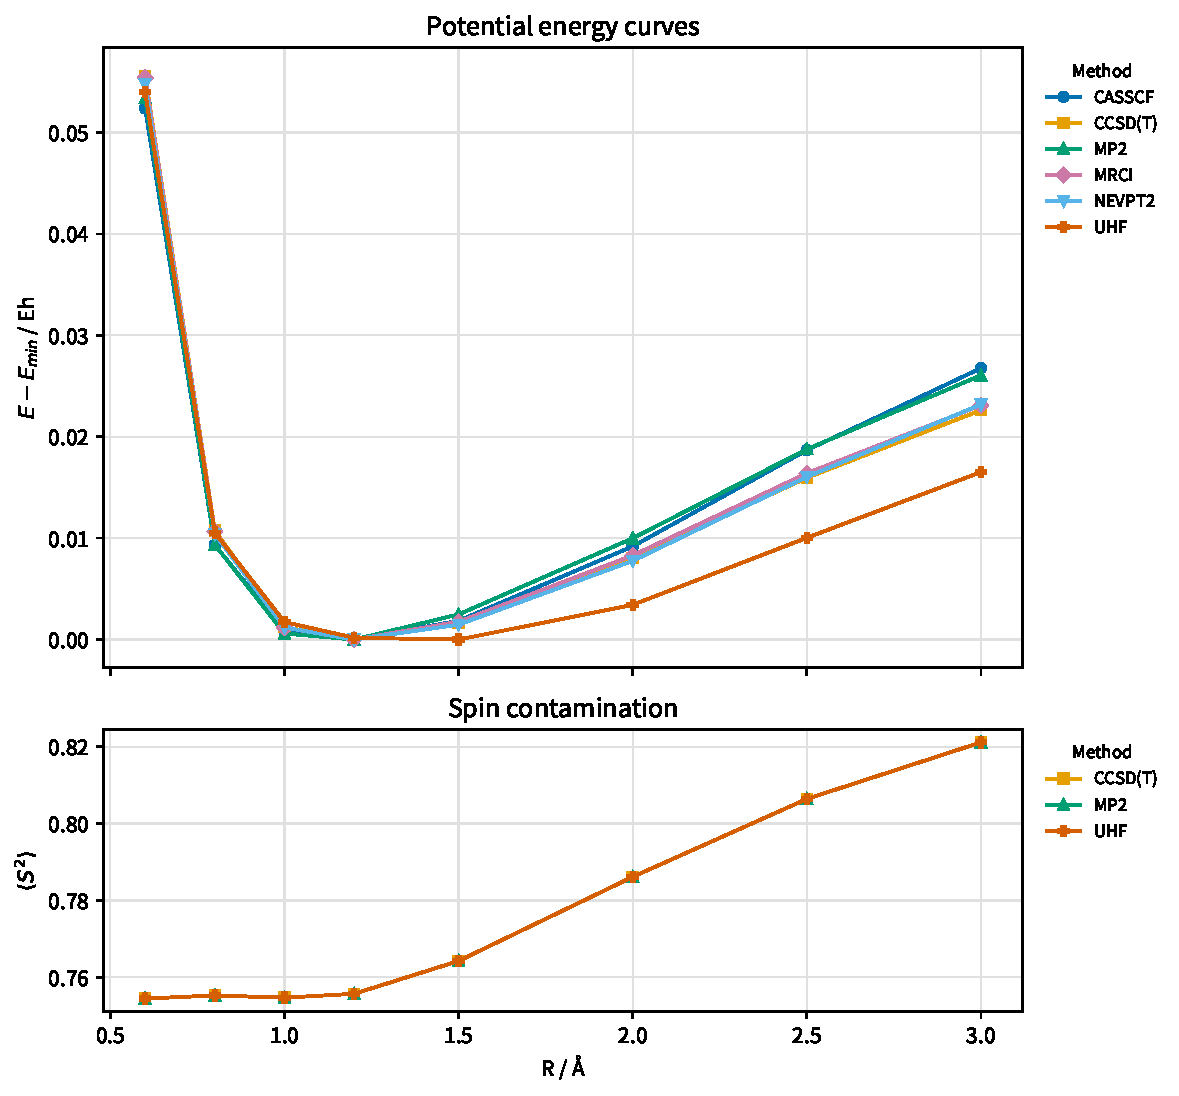
\includegraphics[width=\textwidth]{figures/ch07/h2m_pes.pdf}
\caption{H$_2^-$/def2-TZVPP 的势能曲线（上）与 UHF 的 $\langle S^2\rangle$（下）。
上图的纵轴是各方法自己的 $E-E_{\min}$，只用于比较曲线形状，不能跨方法比较绝对能量；
下图的 $\langle S^2\rangle$ 只由 UHF 参考给出，MP2 与 CCSD(T) 继承同一参考。}
\label{ch:07:fig:h2m}
\end{figure}

表~\ref{ch:07:tab:h2m} 把 UHF 与 CASSCF 的能量、UHF 的 $\langle S^2\rangle$ 以及 CASSCF 的活性空间自然占据数放在一起。最重要的数据事实是：CASSCF(3,2) 在\textbf{每一个} R 上都\textbf{高于} UHF，差值从 0.0012\,Eh（0.6\,\AA）到 0.0131\,Eh（3.0\,\AA）。这不表示 CASSCF“更差”。UHF 允许 $\alpha$ 与 $\beta$ 电子使用不同的空间轨道，变分自由度更大，代价是波函数不再是纯自旋本征态（$\langle S^2\rangle>0.75$）；CAS(3,2) 用两个共同的空间轨道并强制 \texttt{mult 2}，自旋是干净的，但能量会略高。用 CASSCF 与 UHF 的能量高低来判断“谁更可靠”是错误的，二者的变分空间与自旋约束不同。

\begin{table}[t]
\centering
\small
\caption{H$_2^-$/def2-TZVPP 的 UHF 与 CASSCF(3,2) 数据。能量单位 Eh，保留 6 位小数；
占据数取自 \texttt{data/h2m\_occupations.csv}，“偏离”指 $\min(|n_p|,|n_p-2|)$ 的最大值。
CASSCF 不打印 $\langle S^2\rangle$，因为 \texttt{mult 2} 已强制自旋本征态。}
\label{ch:07:tab:h2m}
\begin{tabular}{@{}lcccccc@{}}
\toprule
$R$/\AA & $E_{\mathrm{UHF}}$ & $E_{\mathrm{CASSCF}}$ & $\langle S^2\rangle_{\mathrm{UHF}}$ & $n_1$ & $n_2$ & 偏离 \\
\midrule
0.6 & $-0.934317$ & $-0.933069$ & 0.754473 & 2.0000 & 1.0000 & 1.0000 \\
0.8 & $-0.977755$ & $-0.976123$ & 0.755273 & 2.0000 & 1.0000 & 1.0000 \\
1.0 & $-0.986566$ & $-0.984600$ & 0.754710 & 2.0000 & 1.0000 & 1.0000 \\
1.2 & $-0.988117$ & $-0.985448$ & 0.755706 & 2.0000 & 1.0000 & 1.0000 \\
1.5 & $-0.988296$ & $-0.983600$ & 0.764251 & 2.0000 & 1.0000 & 1.0000 \\
2.0 & $-0.984874$ & $-0.976261$ & 0.786138 & 2.0000 & 1.0000 & 1.0000 \\
2.5 & $-0.978266$ & $-0.966776$ & 0.806405 & 2.0000 & 1.0000 & 1.0000 \\
3.0 & $-0.971787$ & $-0.958695$ & 0.821141 & 2.0000 & 1.0000 & 1.0000 \\
\bottomrule
\end{tabular}
\end{table}

表~\ref{ch:07:tab:h2m} 的占据数是本书必须诚实对待的地方。CAS(3,2) 的自然占据数在\textbf{所有} R 上都是 2.0000 与 1.0000，偏离恒为 1.0000；输出中的 CI 向量是单一组态（\texttt{1.00000 [1]:21}）。也就是说，\texttt{nroots 1} 的 CASSCF(3,2) 基态在这个最小活性空间里是一个\textbf{单一行列式}（在局域轨道表象中），并没有出现 1.5/1.5 那样的分数占据。占据数“偏离 0 或 2”之所以满足 1.0，只是因为单占据活性轨道的占据数本来就是 1.0，这不是分数静态相关的标志。

那么 H$_2^-$ 的多参考证据在哪里？在三处。第一，UHF 的 $\langle S^2\rangle$ 随 R 从 0.754473 增长到 0.821141，增长量 0.066668，远大于 0.02；自旋污染随键拉伸而加重，说明单参考自旋轨道图像在拉伸区失效（7.8 节）。第二，MP2 与 CCSD(T) 在拉伸区的行为异常：它们虽然仍给出更低的能量，但相对 CASSCF 的修正越来越大，且 CCSD(T) 的微扰分母在近简并时不可靠。第三，CASSCF 之上的 NEVPT2 与 MRCI 修正很大：NEVPT2 比 CASSCF 低 0.0331--0.0391\,Eh，MRCI 又比 NEVPT2 低 0.0129--0.0137\,Eh，且在每个 R 上都如此。动态相关修正的规模本身说明 CASSCF 参考态还远未完成，而 1.5/1.5 的静态相关图像必须由更大的活性空间或态平均计算才能显现，不能从这张表的单组态占据数里读出来。

\subsection{UHF 的自旋污染}
\label{ch:07:sec:spin}

H$_2^-$ 是双重态，纯自旋本征态的 $\langle S^2\rangle=0.75$。UHF 波函数不强制这一点，$\alpha$ 与 $\beta$ 轨道可以不同，于是 $\langle S^2\rangle$ 偏离 0.75。表~\ref{ch:07:tab:h2m} 与图~\ref{ch:07:fig:h2m} 的下半部分给出完整序列：0.754473（0.6\,\AA）、0.755273（0.8）、0.754710（1.0）、0.755706（1.2）、0.764251（1.5）、0.786138（2.0）、0.806405（2.5）、0.821141（3.0）。

这组数据有两个必须如实报告的细节。第一，增长不是严格单调的：0.8\,\AA 的 0.755273 比 1.0\,\AA 的 0.754710 高 0.000563，随后才继续上升。这个微小凹陷来自 SCF 收敛路径与轨道近简并的耦合，不影响“拉伸区污染加重”的结论，但不能为了叙事把它抹平。第二，0.75 附近的数值本身已经偏离纯自旋值，说明即使在平衡区附近，UHF 也不是纯双重态；只是到了 3.0\,\AA，偏离才明显放大。MP2 与 CCSD(T) 以 UHF 为参考，因此 CSV 中它们的 $S^2$ 列与 UHF 相同；这不是三个独立证据，而是同一个参考态的自旋污染被三种方法继承。

CASSCF 的情况不同：\texttt{mult 2} 强制波函数是自旋本征态，$\langle S^2\rangle$ 应为 0.75，ORCA 对这类计算不打印 $S^2$，CSV 中 CASSCF/NEVPT2/MRCI 的 $s^2$ 列为空。不能把“空”理解为“没有自旋污染”或“有污染”，它只是这些方法不输出该量；正确说法是自旋对称性由构造保证。

% ---- 4. CH4 结果框 ----
\begin{ch4box}
CH$_4$/def2-TZVPP：$E_{\mathrm{CASSCF}(8,8)} = -40.297163$\,Eh
（CSV 精确值 $-40.297162861153$\,Eh），
$\Delta E = +88.75$\,kcal·mol$^{-1}$（相对 CCSD(T)）。
活性空间自然占据数为 $1.98429$、$1.97895\times3$、$0.01971\times4$，总和 8。
这些数接近 2 与 0，说明 CH$_4$ 只有\textbf{弱}静态相关；它与拉伸 H$_2^-$ 的强近简并不是一回事。
CASSCF 缺掉的动态相关由第 8 章的 CASPT2/NEVPT2/MRCI 补上。
\end{ch4box}

% ---- 5. 常见陷阱 ----
\begin{pitfall}
\begin{itemize}
  \item \textbf{把 CASSCF 当成“自动包含所有相关”}：CASSCF 只包含活性空间内的静态相关；活性空间外的动态相关仍需 CASPT2、NEVPT2 或 MRCI。CASSCF 能量不能当作高精度基准。
  \item \textbf{用能量高低判断 CASSCF 与 UHF 谁更可靠}：UHF 的变分空间更大且允许自旋污染，能量更低并不代表波函数更好；比较必须看 $\langle S^2\rangle$、占据数与后续多参考修正。
  \item \textbf{把态平均结果当基态}：\texttt{nroots 2} 的态平均占据数可能是 1.5/1.5，但那是两个态的平均，不是 \texttt{nroots 1} 的基态；本书 H$_2^-$ 数据全部取 \texttt{nroots 1}。
  \item \textbf{活性空间越大越好}：式~\eqref{ch:07:eq:determinant-count} 的指数增长会让计算不可行；应先按化学直觉与占据数选最小空间，再做收敛性检查。
\end{itemize}
\end{pitfall}

% ---- 6. 小结 + 过渡 ----
\subsection*{小结}
CASSCF 用活性空间内的全 CI 式~\eqref{ch:07:eq:casscf-wavefunction} 容纳近简并组态，并通过式~\eqref{ch:07:eq:orbital-generator}--\eqref{ch:07:eq:orbital-ci-gradient} 把轨道与 CI 系数联合优化；它是变分的、尺寸一致的，但成本随活性空间指数增长（式~\eqref{ch:07:eq:determinant-count}）。H$_2^-$ 的 CAS(3,2) 数据给出了一个诚实的教训：\texttt{nroots 1} 的占据数是 2.0/1.0 而非 1.5/1.5，CASSCF 在能量上还高于 UHF，多参考必要性来自 $\langle S^2\rangle$ 增长与 NEVPT2/MRCI 的大修正，而不是 CASSCF--UHF 的能量排序。CASSCF 仍缺动态相关，这正是下一章要补的。带着这个问题，我们进入第 8 章：CASPT2/NEVPT2/MRCI：如何给多参考态补动态相关？
